%%%%%%%%%%%%%%%%%%%%%%%%%%%%%%%%%%%%%%%%%%%%%%%%%%%%%%%%%%%%%%%%%
% Contents: No Input Device
% $Id: typeset.tex 537 2015-07-18 09:43:10Z oetiker $
%%%%%%%%%%%%%%%%%%%%%%%%%%%%%%%%%%%%%%%%%%%%%%%%%%%%%%%%%%%%%%%%%
\renewcommand{\chaptername}{Section}
\chapter{REMOVE THIS LATER}

OLD STUFF FROM PREVIOUS ITERATIONS OF MM. DONT FORGET TO REMOVE

  In order to change the sequencer mode and order, first access the Menu Page
  by hitting the bottom-left circular button on the \emph{Manta}.

  \begin{figure}[h!]
    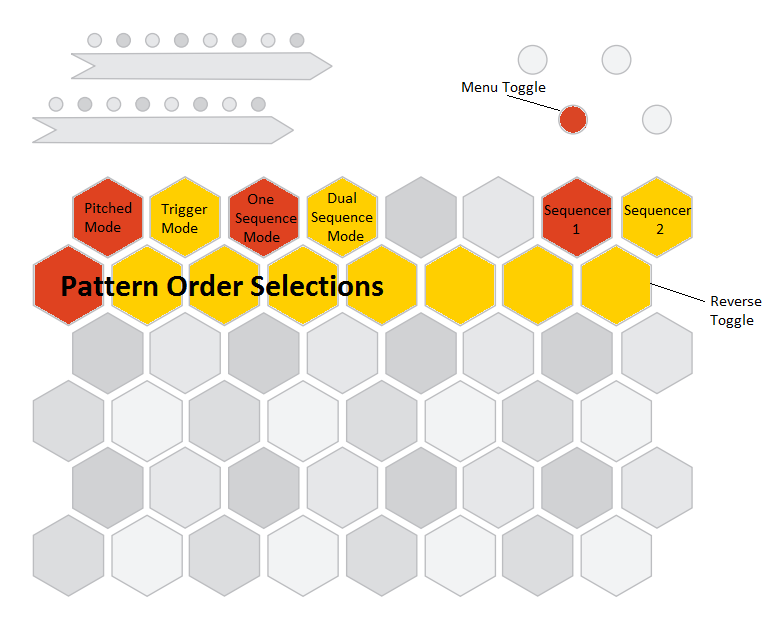
\includegraphics[width=\linewidth]{menu.png}
  \end{figure}

  There are four (TODO: Five?) sequencer modes the Manta can be in that are accessed by the
  the top-left four Hexes in the Menu Page:

  From left to right:
  \begin{itemize}
    \item Pitched (default)
    \item Dual-Sequence Pitched
    \item Trigger
    \item Dual-Sequence Trigger
    \item Mixed (TODO?)
  \end{itemize}

  Although the naming seems to imply otherwise, both Pitched Mode and
  Dual-Sequence Pitched Mode have two running sequences. The difference
  lies in that the Dual-Sequence Pitched Mode presents the user both
  sequences on the same page, while the two sequences in Pitched Mode must
  be flipped between using the two rightmost hexes in the Menu Page.

  The above is also true of Trigger Mode and Dual-Sequence Trigger Mode.

  The Menu Page also allows you to switch the sequence order mode,
  these can be changed by the second row of hexes:

  From left to right:
  \begin{itemize}
    \item Left to right, bottom to top
    \item Left to right, top to bottom
    \item Diagonally up
    \item Diagonally down
    \item Caterpillar
    \item Order in which hexes are added
    \item Random
    \item Reverse the currently selected order mode. Or turn random mode to
    a random walk pattern.
  \end{itemize}


% Local Variables:
% TeX-master: "lshort2e"
% mode: latex
% mode: flyspell
% End:
